In order to implement the application, first of all, a new project has to be created in Eclipse. This project is going to be a Papyrus project (figure \ref{fig:Papyrus Project}).

\begin{figure}
\centering
{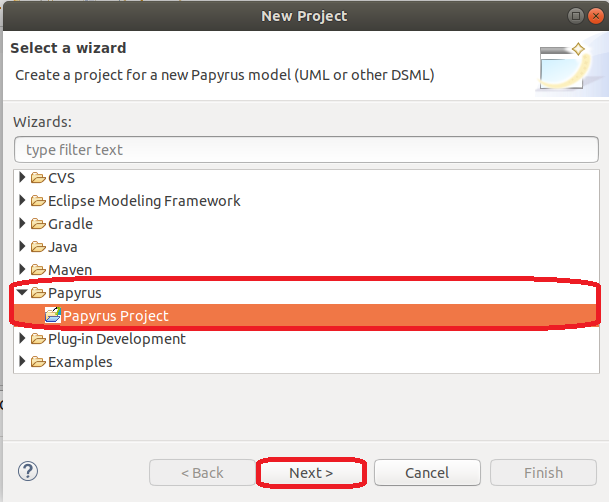
\includegraphics[scale=0.3]{./chapter4/projPapyrus/Selection_001.png}}
\caption{New Papyrus Project}
\label{fig:Papyrus Project}
\end{figure}

The first field that has to be specified is the Architecture Context. Here, the default values are the right ones as an UML model is what is required to implement with Papyrus (figure \ref{fig:Architecture Context}).

\begin{figure}
\centering
{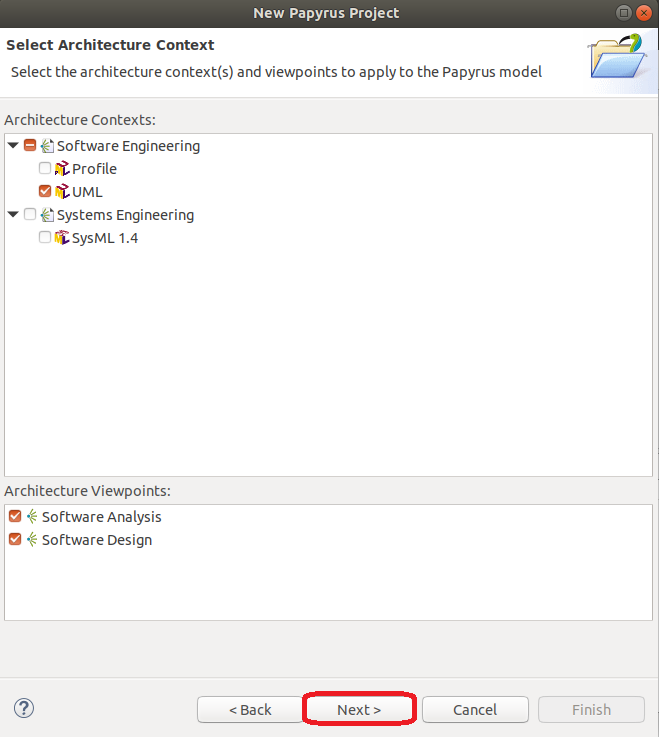
\includegraphics[scale=0.3]{./chapter4/projPapyrus/Selection_002.png}}
\caption{Architecture Context}
\label{fig:Architecture Context}
\end{figure}

After that, the name of the project has to be defined. Due to the fact that it is going to implement an application called Great Seller, the name of the Papyrus project is going to be greatSellerApp (figure \ref{fig:Project Name Definition}).

\begin{figure}
\centering
{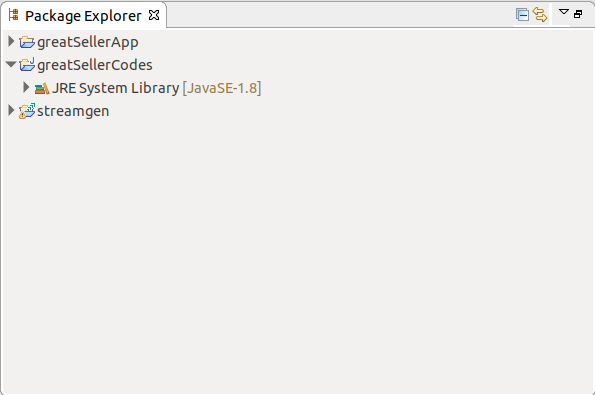
\includegraphics[scale=0.3]{./chapter4/projPapyrus/Selection_003.png}}
\caption{Project Name Definition}
\label{fig:Project Name Definition}
\end{figure}

The next step is to select the representation kind and to choose the StreamGen profile. StreamGen requires Papyrus to make a class diagram representation and, as the StreamGen project is already in the Eclipse workspace, the profile can be found browsing in the workspace (streamgen/profile/StreamUML.profile.uml). As it can be seen in the figure \ref{fig:Representation Kind}.

\begin{figure}
\centering
{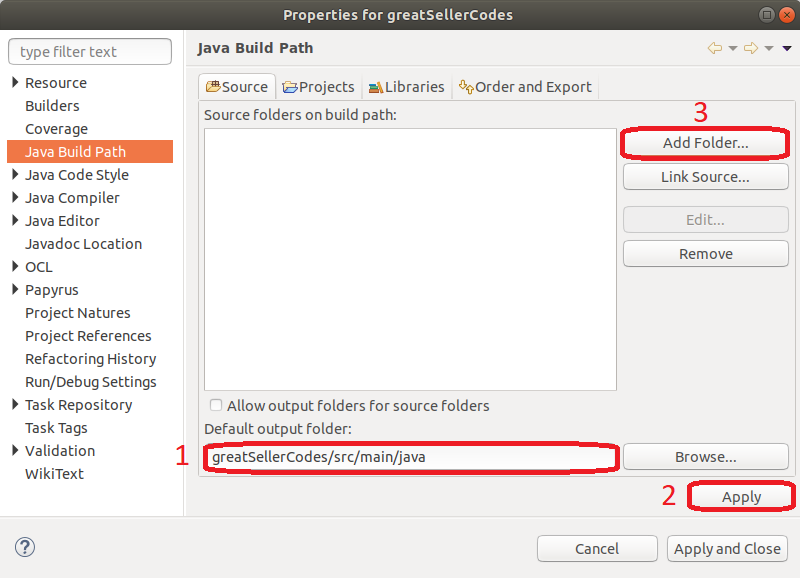
\includegraphics[scale=0.3]{./chapter4/projPapyrus/Selection_004.png}}
\caption{Representation Kind}
\label{fig:Representation Kind}
\end{figure}

Finally, we can finish with the new Papyrus project initialization (figure \ref{fig:Papyrus Project Definition}).

\begin{figure}
\centering
{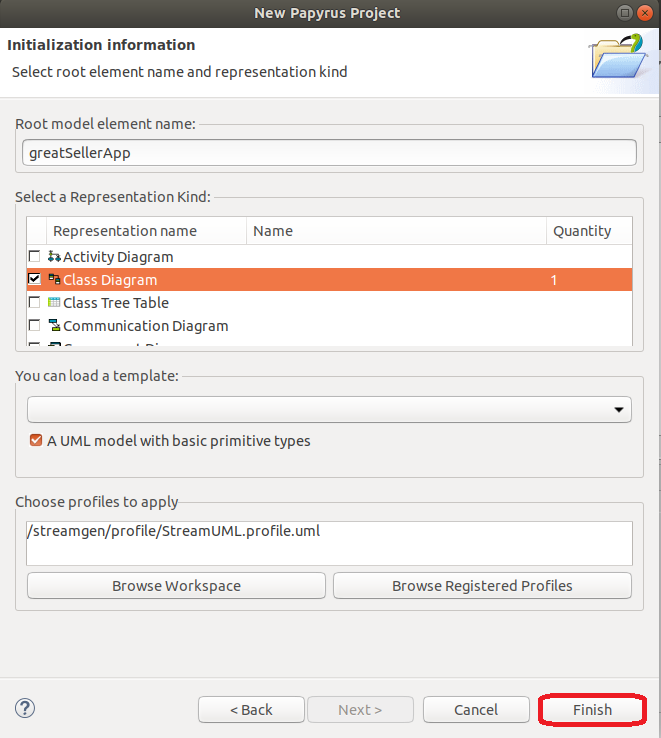
\includegraphics[scale=0.3]{./chapter4/projPapyrus/Selection_005.png}}
\caption{Papyrus Project Definition}
\label{fig:Papyrus Project Definition}
\end{figure}

The next step is to define the model in the class diagram in order to specify that the application is going to be a Flink application. Then, first of all, we have to create a model node in the greatSellerApp.di file. This node is going to be called greatSeller as it is the object representing the whole application. Once the node is inserted, the properties of such node must be specified. More in detail, the Flink application stereotype has to be applied. In this case, the properties of the model has to be the default ones then nothing else must be done with the model node.

The next step is to add the data types that the application is going to need. In order to do this, a package node has to be inserted inside the Flink application model node. This package is called greatSellerDataTypes and a stereotype has to be applied as in the previous case. First of all, inside the properties windown, in the profile field, the applied stereotype is defined. Inside this package all the datatypes that the application requires have to be inserted. The first data type is the InputTransactions which is composed of a transaction id (integer), a data subject (string), an amount (double) and a recipient id (string). The second data type is the IssuedTransactions which contains the data subject (string) and the number of transactions performed by such data subject which can be seen by means of the variable NTransactions (integer). The third data type is the SpentAmount which is composed of the data subject (string) and the total amount of money spent by the data subject which can be seen by means of the variable TotalAmount (double). Finally, the last data type is the NumberUsers which contains the number of users who spent more than 1000 dollars and it is represented by means of the variable NTopUsers (integer). Then, we need to insert one DataType node inside the package created in the previous step with each of these data types. Each data type can be seen as a tuple which is composed by several values. The name of the DataType node is going to be the same that the one corresponding to the tuple and each of the values that compose the tuple are going to be a property inside of the owned attributes that are specified in the UML field of the properties of each DataType node.

\begin{table}[h!]
\centering
	\begin{tabular}{||c|c|c||} 
	\hline\hline
	DataType & Properties & PropertyType \\ [1ex] 
	\hline\hline
	InputTransactions & transactionId & integer  \\
	& dataSubject & string  \\
	& amount & double  \\
	& recipientId & string  \\
	\hline
	IssuedTransactions & dataSubject & string  \\
	& nTransactions & integer \\
	\hline
	SpentAmount & dataSubject & string  \\
	& totalAmount & double \\
	\hline
	NumberUsers & NTopUsers & double  \\
	\hline\hline
	\end{tabular}
\caption{DataTypes Composition}
\label{DataTypes Composition}
\end{table}
